\documentclass[11pt]{article}
\usepackage[final]{acl}
\usepackage{times}
\usepackage{multirow}
\usepackage{latexsym}
\usepackage[T1]{fontenc}
\usepackage[utf8]{inputenc}
\usepackage{microtype}
\usepackage{inconsolata}
\usepackage{amsmath}
\usepackage{amssymb}
\usepackage{booktabs}
\usepackage{enumitem}
\usepackage{graphicx}
\usepackage{listings}
\usepackage{tikz}
\usepackage{xcolor}

\setlist[itemize]{noitemsep,topsep=2pt,leftmargin=*}
\setlist[enumerate]{noitemsep,topsep=2pt,leftmargin=*}

\lstset{
  basicstyle=\ttfamily\scriptsize,
  breaklines=true,
  breakatwhitespace=false,
  frame=single,
  framesep=2pt,
  columns=fullflexible,
  keepspaces=true,
  xleftmargin=2pt,
  xrightmargin=2pt,
  aboveskip=4pt,
  belowskip=4pt,
  escapeinside={(*@}{@*)},
}


\usetikzlibrary{positioning, arrows.meta, fit, backgrounds, shapes.geometric, calc}


\title{AILS-NTUA at SemEval-2026 Task 10: Agentic LLMs for Psycholinguistic Marker Extraction and Conspiracy Endorsement Detection}


\author{Panagiotis Spanakis \hspace{0.8em} Maria Lymperaiou \hspace{0.8em} Giorgos Filandrianos \\
Athanasios Voulodimos \hspace{0.8em} Giorgos Stamou \\
National Technical University of Athens (NTUA)}

\begin{document}
\maketitle
\begin{abstract}
    This paper describes an agentic LLM system for SemEval-2026 Task 10 that jointly (i) extracts psycholinguistic conspiracy markers as text spans and (ii) classifies whether a Reddit comment endorses a conspiracy.
    The design separates semantic extraction from deterministic span localization and uses an Anti-Echo Chamber council to reduce false positives on reporting/debunking content.
\end{abstract}

\section{Introduction}
Humans have long exhibited a tendency to endorse conspiracy theories,
particularly in contexts of uncertainty, threat, and social upheaval. Such
beliefs are created and distributed to support human need for addressing
existential or social issues and strengthen their sense of identity and
belonging \cite{psychology-of-conspiracy, belief}. Despite their psychological
appeal, conspiracies are associated with harmful consequences, limiting trust
in well-documented facts and public decisions, while exacerbating political
polarization and misinformation patterns \cite{understanding}.

The rise of artificial intelligence inspired the connection of conspiracy
identification with natural language, as language constitutes the most
fundamental medium for conspiracy articulation and spread. Conspiratorial
statements are subtly embedded in language exploiting linguistic strategies to
evoke emotions and attribution of agency \cite{miani2022loco,
    rains2023psycholinguistic}, suggesting that conspiracy identification goes well
beyond superficial linguistic cues.

Large Language Models (LLMs) have revolutionized linguistic research, enabling
deep pattern identification and discrimination among their numerous abilities.
However, LLMs have been found to be significantly prone to cognitive biases
\cite{filandrianos-etal-2025-bias} and manipulation via persuasive language
\cite{xu-etal-2024-earth}, while they generate and amplify misinformation
\cite{chen2024combatingmisinformation}. Going one step further,
state-of-the-art LLMs are even able to persuade people to adopt conspiratorial
beliefs to a comparable degree as they can mitigate conspiracy dissemination
\cite{costello2026largelanguagemodelseffectively}, exposing the double-edged
nature of LLMs in the context of factual verification.

The core challenges that conspiratorial discourse poses call for fine-grained
data approaches that allow delving into the linguistic mechanisms that
characterize conspiratorial utterances in an interpretable way. Nevertheless,
prior datasets \cite{shahsavari2020conspiracy, langguth2023coco} frame
conspiracy detection as a coarse-grained classification task, abstracting away
from the particularities of conspiratorial discourse, thus obscuring how
conspiratorial reasoning is formed and expressed in language. To fill this gap,
the \textbf{SemEval 2026 Task 10: Psycholinguistic Conspiracy Marker Extraction
    and Detection} emphasizes the localization and categorization of linguistic
markers that signal conspiratorial thinking, complementing detection with
psychologically-backed annotations.

To address the dual challenges of accurate detection and interpretable marker
extraction, models must be capable of capturing both global conspiratorial
intent and fine-grained psycholinguistic cues embedded in language. In our
approach, we leverage LLMs within agentic structures to advance the recognition
of conspiratorial thought. Specifically, [] To the best of our knowledge, we
introduce the \textit{first agentic LLM-based method} to combat conspiracy
detection and identification of psycholinguistic features in language.

In short, our contributions are the following:
\begin{itemize}
    \item We introduce the first agentic LLM-based method for psycholinguistic conspiracy
          marker extraction and detection.
\end{itemize}

\section{Background}
\paragraph{Task description}
The dataset comprises 4,800 annotations spanning 4,100 unique Reddit submission
statements from $>$190 subreddits, divided in two subtasks: \textbf{\textit{i)}
    S1: Conspiracy Marker Extraction} contains textual spans that express core
conspiracy markers grounded in evolutionary psychology. One or more marker
types may appear in each comment, falling in the following categories:
\textsc{Actor} (mentions of individual or group agents), \textsc{Action}
(descriptions of what the actor is doing), \textsc{Effect} (consequences of the
actions), \textsc{Victim} (who is being harmed), \textsc{Evidence} (claims or
proof used to support the theory). \textbf{\textit{ii)} S2: Conspiracy
    Detection} assigns conspiracy-related or not conspiracy-related labels to
Reddit comments. More details about the dataset are provided in App.
\ref{sec:eda}.

\paragraph{Related work}
Early works on NLP conspiratorial discourse on Reddit introduced narrative
motifs correlated with conspiratorial evidence \cite{online-discussions} and
demonstrated that conspiratorial thinking manifests through detectable
psycholinguistic signals in user language \cite{Klein2019Pathways}, with
consequent literature revealing that conspiracy theories exhibit distinctive
narrative frameworks that can be computationally extracted from text
\cite{Tangherlini2020Automated}. These foundational works empowered the
operationalization of conspiracy identification as a classification task,
exemplified by datasets such as COCO \cite{langguth2023coco} and YouNICon
\cite{YouNICon}. Conspiracy detection involves techniques that explicitly model
psycholinguistic signals, such as affective tone, attributional cues and
explanatory framing, in order to provide explanatory evidence of conspiracy
presence in language \cite{rains2023psycholinguistic,
    language-of-conspiracy-theories, marino-etal-2025-linguistic}. The strong
contextualization that LLMs offer inspired the introduction of related
approaches; leveraging appropriate prompting enables accurate multi-label
conspiracy classification, eliminating training demands
\cite{peskine-etal-2023-definitions}. Complementarily, ConspEmoLLM
\cite{liu2024conspemollm} involves emotion-aware LLM fine-tuning on several
conspiratorial tasks, improving detection by leveraging affective signals, with
subsequent extensions focusing on robustness to stylistic and emotional
variation \cite{liu2025conspemollmv2}. Recent evaluations indicate that
LLM-based conspiracy detection often relies on topical shortcuts and struggles
with narrative ambiguity, underscoring the need for approaches grounded in
interpretable psycholinguistic markers \cite{pustet-etal-2024-detection,
    classifying}.

\section{System Overview}

We implement a two-stage agentic workflow: \textbf{S1}
extracts psycholinguistic marker spans, and \textbf{S2} predicts conspiracy
endorsement conditioned on the document and the extracted markers. The design
separates (i) LLM-mediated semantic decisions (what to extract / how to
interpret stance) from (ii) deterministic operations that require exactness
(character offsets, lightweight text statistics). Figure~\ref{fig:arch}
summarizes the inference flow.

\begin{figure*}[t]
    \vspace{-6pt}
    \centering
    \scriptsize
    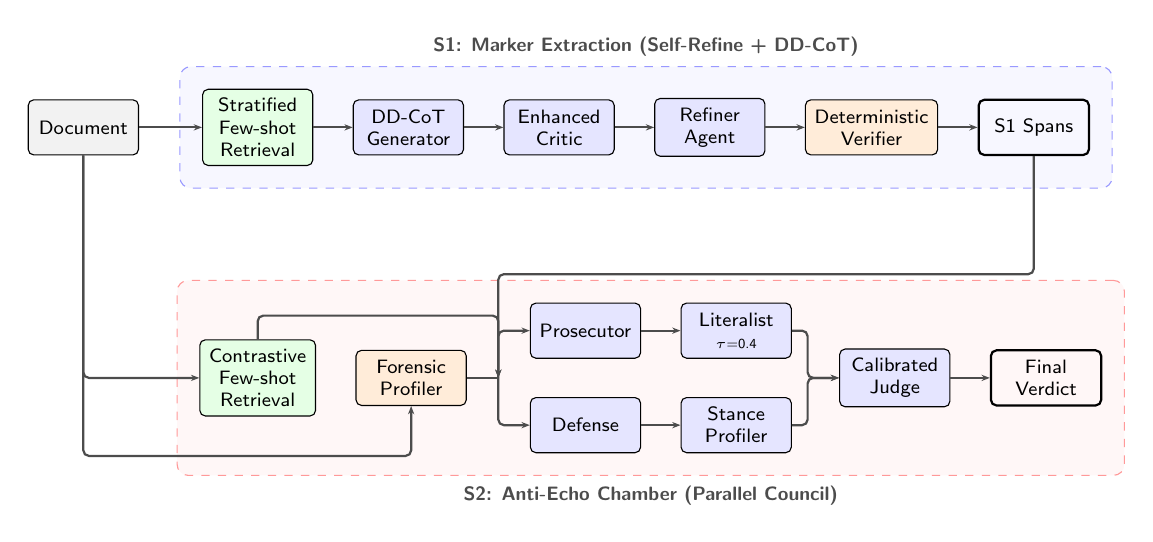
\begin{tikzpicture}[
        node distance=0.6cm and 0.4cm,
        >={Stealth[length=3pt]},
        % Styles
        inputbox/.style={rectangle, draw, rounded corners=2pt, minimum height=0.7cm,
                minimum width=1.4cm, align=center, font=\scriptsize\sffamily, fill=gray!10},
        ragbox/.style={rectangle, draw, rounded corners=2pt, minimum height=0.7cm,
                minimum width=1.4cm, align=center, font=\scriptsize\sffamily, fill=green!10},
        llmbox/.style={rectangle, draw, rounded corners=2pt, minimum height=0.7cm,
                minimum width=1.4cm, align=center, font=\scriptsize\sffamily, fill=blue!10},
        detbox/.style={rectangle, draw, rounded corners=2pt, minimum height=0.7cm,
                minimum width=1.4cm, align=center, font=\scriptsize\sffamily, fill=orange!15},
        outputbox/.style={rectangle, draw, rounded corners=2pt, minimum height=0.7cm,
                minimum width=1.4cm, align=center, font=\scriptsize\sffamily, thick},
        arrow/.style={->, thick, black!70, rounded corners=2pt}, dasharrow/.style={->,
                thick, dashed, black!50, rounded corners=2pt},
        grouplab/.style={font=\bfseries\scriptsize\sffamily, text=black!70},
        labeltext/.style={font=\tiny\sffamily, text=black!60, midway, fill=white, inner
                sep=1pt}, ]

        % === INPUT ===
        \node[inputbox] (input) {Document};

        % === S1 PIPELINE (Top Row) ===
        \node[ragbox, right=0.8cm of input] (s1rag) {Stratified\\Few-shot\\Retrieval};
        \node[llmbox, right=0.5cm of s1rag] (gen) {DD-CoT\\Generator};
        \node[llmbox, right=0.5cm of gen] (critic) {Enhanced\\Critic};
        \node[llmbox, right=0.5cm of critic] (refiner) {Refiner\\Agent};
        \node[detbox, right=0.5cm of refiner] (verifier) {Deterministic\\Verifier};
        \node[outputbox, right=0.5cm of verifier] (s1out) {S1 Spans};

        % S1 Connections
        \draw[arrow] (input) -- (s1rag);
        \draw[arrow] (s1rag) -- (gen);
        \draw[arrow] (gen) -- (critic);
        \draw[arrow] (critic) -- (refiner);
        \draw[arrow] (refiner) -- (verifier);
        \draw[arrow] (verifier) -- (s1out);

        % S1 Group Label
        \begin{scope}[on background layer]
            \node[draw=blue!40, fill=blue!3, rounded corners=4pt, dashed,
            fit=(s1rag)(gen)(critic)(refiner)(verifier)(s1out),
            inner sep=8pt, label={[grouplab]above:{S1: Marker Extraction (Self-Refine + DD-CoT)}}] (s1group) {};
        \end{scope}

        % === S2 PIPELINE (Bottom Row) ===
        \node[ragbox, below=2.2cm of s1rag] (s2rag) {Contrastive\\Few-shot\\Retrieval};
        \node[detbox, right=0.5cm of s2rag] (forensic) {Forensic\\Profiler};

        % PARALLEL COUNCIL (Strict 2x2 Grid)
        \node[llmbox, right=0.8cm of forensic, yshift=0.6cm] (pros) {Prosecutor};
        \node[llmbox, right=0.5cm of pros] (literal) {Literalist\\{\tiny $\tau$=0.4}};

        \node[llmbox, right=0.8cm of forensic, yshift=-0.6cm] (defense) {Defense};
        \node[llmbox, right=0.5cm of defense] (profiler) {Stance\\Profiler};

        % Judge
        \node[llmbox, right=0.6cm of $(literal.east)!0.5!(profiler.east)$] (judge) {Calibrated\\Judge};
        \node[outputbox, right=0.5cm of judge] (verdict) {Final\\Verdict};

        % Fork (Clean Distribution)
        \coordinate[right=0.4cm of forensic] (fork_point);
        \draw[thick, black!70] (forensic.east) -- (fork_point);
        \draw[arrow] (fork_point) |- (pros.west);
        \draw[arrow] (fork_point) |- (defense.west);

        % S2 Connections
        \draw[arrow] (input.south) |- (s2rag.west);
        \draw[arrow] (input.south) |- ($(s2rag.south) + (0,-0.5)$) -| (forensic.south);

        % S1 Out to Council 
        \draw[arrow] (s1out.south) -- ++(0,-1.5) -| (fork_point);

        % S2RAG to Council (Bypassing Forensic)
        \draw[arrow] (s2rag.north) -- ++(0,0.3) -| (fork_point);

        % Internal Flow
        \draw[arrow] (pros) -- (literal);
        \draw[arrow] (defense) -- (profiler);

        % Merge (Clean Join)
        \draw[arrow] (literal.east) -- ++(0.2,0) |- (judge.west);
        \draw[arrow] (profiler.east) -- ++(0.2,0) |- (judge.west);
        \draw[arrow] (judge) -- (verdict);

        % S2 Group Label
        \begin{scope}[on background layer]
            \node[draw=red!40, fill=red!3, rounded corners=4pt, dashed,
            fit=(s2rag)(forensic)(pros)(defense)(literal)(profiler)(judge)(verdict),
            inner sep=8pt, label={[grouplab]below:{S2: Anti-Echo Chamber (Parallel Council)}}] (s2group) {};
        \end{scope}

    \end{tikzpicture}
    \vspace{-4pt}
    \caption{System architecture overview. \textbf{S1} (top): DD-CoT Self-Refine extracts marker strings, then a deterministic verifier anchors them to character offsets. \textbf{S2} (bottom): an Anti-Echo Chamber (forensic profiling + parallel council + calibrated judge) predicts conspiracy endorsement.}
    \label{fig:arch}
    \vspace{-10pt}
\end{figure*}

\subsection{S1: Marker Extraction via DD-CoT}

S1 produces a set of labeled spans by combining a self-refinement loop with a
deterministic span locator. The graph consumes the document and retrieved
few-shot precedents, generates candidate marker \emph{strings} with labels,
iteratively corrects them, then anchors each string to \texttt{startIndex} and
\texttt{endIndex} in the original text.

\paragraph{Hybrid Architecture Rationale.} We explicitly decouple \textit{semantic identification} from \textit{span
    indexing}. LLMs can justify category assignments but are brittle at
character-accurate localization \cite{fu2024struggle}. We therefore (i) ask the
LLM to emit verbatim marker strings with labels, and (ii) compute offsets with
a deterministic locator that performs exact matching against the source text.
This avoids ``hallucinated spans'' and off-by-one indices while preserving the
LLM's interpretive signal \cite{ogasa-arase-2025-hallucinated}.

\paragraph{Dynamic Discriminative Chain-of-Thought (DD-CoT).} DD-CoT extends CoT reasoning \cite{wei2022chain} with an explicit
\emph{discrimination step}. For each candidate span, the generator must state
(i) evidence for the chosen label and (ii) a short counter-argument against at
least one confusable label. This forces the model to commit to a decision
boundary in frequent confusions (e.g., \textsc{Actor} vs. \textsc{Victim},
\textsc{Action} vs.\ \textsc{Effect}) rather than producing post-hoc
rationales.

\paragraph{Agents} The Self-Refine loop comprises four sequential nodes: (i)~a DD-CoT
\textbf{Generator} that proposes labeled marker strings; (ii)~an
\textbf{Enhanced Critic} that checks verbatimness, boundaries, label
discrimination, and missing spans; (iii)~a \textbf{Refiner} that applies
minimal edits; and (iv)~a \textbf{Deterministic Verifier} that maps strings to
character offsets and deduplicates overlaps. The verifier's matching cascade is
detailed in Appendix~\ref{app:verifier}.

\paragraph{Self-Refine} follows the standard critique--revise pattern \cite{madaan2023selfrefine} but
operates over typed intermediate artifacts (candidate spans, critiques, and
edits), improving controllability and enabling deterministic verification.

\subsection{S2: Classification via Anti-Echo Chamber}

S2 targets a specific failure mode: \textbf{Reporter Trap} false positives, in
which topical discussion of conspiracies is conflated with endorsement (e.g.,
reporting, debunking, satire). Single-pass classifiers often over-commit early
and underweight stance cues \cite{wan-etal-2025-unveiling}. We therefore
structure S2 as: (i) a deterministic \emph{Forensic Profiler} that emits
stance-relevant warnings; (ii) a \emph{Parallel Council} that produces
independent pro/contra analyses; and (iii) a \emph{Calibrated Judge} that
aggregates votes with conservative confidence rules.

\paragraph{Forensic Profiler.}
Before LLM deliberation, a deterministic node computes lightweight linguistic
signals (e.g., attribution/reporting cues, shouting/affect, question-heavy
``JAQing'' (``just asking questions'') patterns) that are injected as structured warnings. Full metric
definitions are provided in Appendix~\ref{app:forensic}.

%\paragraph{Forensic Profiler (Static Analysis).} Before LLM deliberation, a deterministic profiling node computes linguistic signatures: (i) \textit{Attribution Density}---frequency of distancing verbs (``said'', ``claimed'', ``according to'') that signal reporting vs.\ endorsement; (ii) \textit{Shouting Score}---proportion of ALL-CAPS tokens (excluding single letters and acronyms); (iii) \textit{JAQing Detection}---high question density combined with hedging terms suggesting ``Just Asking Questions'' manipulation; (iv) \textit{Agency Gap}---passive voice frequency indicating hidden hands. These metrics are injected into council prompts as contextual warnings.

\paragraph{Parallel Council Architecture.} The \textbf{Anti-Echo Chamber} enforces independent assessment by four personas
that receive identical inputs (document, S1 markers, retrieval context,
profiler warnings) and produce structured votes without seeing each other's
outputs:
\begin{enumerate}
    \item \textbf{Prosecutor:} evidence \emph{for} endorsement.
    \item \textbf{Defense Attorney:} evidence \emph{against} endorsement (reporting/debunking/satire cues).
    \item \textbf{Literalist:} literal entailment and burden-of-proof checks.
    \item \textbf{Profiler:} stance cues (certainty, framing, group dynamics).
\end{enumerate}

Each juror outputs: (i) a verdict with confidence, (ii) the primary evidence
supporting that verdict, (iii) a mandatory counter-argument, and (iv)
uncertainty flags for known ambiguities (e.g., reporting vs.\ endorsing,
sarcasm). This design reduces information leakage and ordering effects typical
of sequential debate.

\paragraph{Calibrated Judge.} The Judge aggregates votes and applies conservative confidence rules. We
compute a weighted score $$W = \sum_{j=1}^{4} \begin{cases} +c_j & \text{if } v_j = \texttt{conspiracy} \\ -c_j & \text{if } v_j = \texttt{non} \end{cases}$$
with equal persona weights, where $c_j \in [0,1]$ is juror confidence and $v_j$
its verdict. The Judge consumes the full vote transcript and summary
statistics (e.g., consensus and shared uncertainty flags) and can incorporate
lightweight contextual priors (e.g., \textsc{Conspiracy Hub} subreddit tags).
When the council splits ($2$--$2$), we cap confidence at $0.75$, mark the case
\texttt{borderline}, and default to \texttt{non} when evidence remains
ambiguous. Overrides of a non-split majority are explicitly flagged.

\subsection{Contrastive Few-shot Retrieval}
\label{sec:contrastive-rag}
In-context few-shot examples are retrieved for the given document (no augmentation
is performed). A contrastive strategy is optionally used to supply
discriminative precedents (including hard negatives for the Reporter Trap).
For S1, retrieval is additionally \emph{stratified}: we balance positive/negative documents and upweight underrepresented marker types (e.g., \textsc{Evidence}, \textsc{Victim}) so that prompts include instructive cases beyond the dominant \textsc{Actor}/\textsc{Action} patterns.
For S2, hard negatives are \texttt{non} documents that nevertheless contain S1
marker vocabulary; they match topic but oppose stance, forcing deliberation to
attend to attribution, hedging, and framing cues rather than topical overlap.
This targets Reporter Trap errors by construction.
Full retrieval specification, weights, reranking, and Figure~\ref{fig:rag} are
preserved in Appendix~\ref{app:rag-details}.

\section{Experimental Setup}

We follow the official SemEval train/dev splits without modification; we report
results on the provided dev set (\textit{100} documents) and the official test
set (\textit{938} documents). The primary baseline is a zero-shot GPT-5.2
classifier/extractor using a single prompt (no retrieval, no self-refinement,
no council). Our system uses the same base model but adds workflow structure
and contrastive retrieval.

During early development we used Claude Sonnet 4.5 for rapid prompt iteration.

\paragraph{Contrastive sampling.} Retrieval draws in-context examples from a vector store with reranking, with an
emphasis on \emph{contrast} rather than similarity for S2. In particular, we
explicitly mine and retrieve hard negatives (\texttt{non} documents containing
S1 markers) to expose the stance boundary that drives Reporter Trap false
positives.

\paragraph{GEPA optimization.} Prompt templates were optimized with GEPA \cite{agrawal2025gepa}
(Appendix~\ref{sec:gepa-details}). We used a population of 20--30 prompts over
40--80 generations with tournament size 3, mutation rate 0.2, and GPT-5.2 for
semantic crossover and reflective mutation. S1 fitness is macro $F_2$
(\S\ref{sec:gepa-fitness}); S2 fitness uses Gradient Consensus (vote-ratio
scoring). Hyperparameters are summarized in Table~\ref{tab:gepa-config}.

All agent nodes use GPT-5.2 with schema-constrained generation via PydanticAI
\cite{pydanticai2024} and are orchestrated via LangGraph \cite{langgraph2024};
full implementation and preprocessing details are in
Appendix~\ref{app:exp-details}.

\paragraph{Evaluation.}
Macro F1 is reported for S1 and macro F1/accuracy for S2; additional
diagnostics (e.g., false positive rate on hard negatives) are reported where
relevant.

\section{Results and Analysis}

\subsection{Main Results}
\label{sec:main_results}

Table~\ref{tab:main_results} compares our workflow against a zero-shot GPT-5.2
baseline on dev and test. The gains are largest on dev, where ablations
quantify which inductive biases contribute most to the improvement.

\begin{table}[h!]
    \centering
    \small
    \setlength{\tabcolsep}{4pt}
    \begin{tabular}{@{}l l r r r@{}}
        \toprule
        \textbf{Task} & \textbf{Split}      & \textbf{Baseline F1} & \textbf{Agentic} & \textbf{$\Delta$} \\
        \midrule
        \multirow{2}{*}{S1}
                      & Dev (\textit{100})  & 0.12                 & \textbf{0.24}    & +100\%            \\
                      & Test (\textit{938}) & --                   & \textbf{0.21}    & --                \\
        \midrule
        \multirow{2}{*}{S2}
                      & Dev (\textit{100})  & 0.53                 & \textbf{0.79}    & +49\%             \\
                      & Test (\textit{938}) & --                   & \textbf{0.75}    & --                \\
        \bottomrule
    \end{tabular}
    \caption{Main results (macro F1). Baseline: zero-shot GPT-5.2. Document counts in parentheses.}
    \label{tab:main_results}
\end{table}

For context, the task organizers' starter-pack baselines report
\textasciitilde0.15 \emph{overlap} $F_1$ for S1 and \textasciitilde0.76
\emph{weighted} $F_1$ for S2 on the dev set
\cite{semeval26_task10_starter_pack}; these scores are not directly comparable
to the macro-$F_1$ numbers in Table~\ref{tab:main_results}.

\textbf{S1: Marker Extraction.} The baseline underperforms because it must
jointly (i) decide category membership and (ii) produce exact span strings and
offsets in one step. The agentic pipeline improves dev macro F1 from 0.12 to
0.24 by separating these responsibilities and iterating with targeted critique
and deterministic verification.

\textbf{S2: Conspiracy Detection.} The dev macro F1 gain (from 0.53 to 0.79) is driven by improved handling of stance ambiguity. In particular,
council deliberation increases recall, while contrastive retrieval reduces
Reporter Trap false positives by supplying topic-matched non-endorsement
examples.

\subsection{Ablation Studies}
\label{sec:ablation}

The primary ablation findings are consolidated into a single compact table;
full breakdowns are preserved in Appendix~\ref{app:ablation-full}.

\begin{table}[t]
    \centering
    \scriptsize
    \setlength{\tabcolsep}{3pt}
    \begin{tabular}{@{}p{3.05cm}p{1.85cm}rrr@{}}
        \toprule
        \textbf{Component / Change}       & \textbf{Metric} & \textbf{Base} & \textbf{New} & \textbf{$\Delta$} \\
        \midrule
        \textbf{S1 Self-Refine}                                                                                \\(Gen + Critic + Refiner) & Macro F1 (dev) & 0.173 & 0.240 & +0.067 \\
        \textbf{S1 DD-CoT}                                                                                     \\(agency) & Actor F1 (dev) & -- & -- & +2.7 pts \\
        \textbf{S1 Retrieval}                                                                                  \\(naive vs none) & Macro F1 (dev) & 0.329 & 0.296 & $-$0.033 \\
        \textbf{S2 Parallel Council}                                                                           \\(vs single) & Recall (dev) & 0.481 & 0.560 & +0.079 \\
        \textbf{S2 Judge}                                                                                      \\(vs majority vote) & Macro F1 (dev) & 0.638 & 0.681 & +0.043 \\
        \textbf{S2 Contrastive Retrieval} & FP rate (dev)   & 0.160         & 0.080        & $-$50\%           \\
        \bottomrule
    \end{tabular}
    \caption{Combined ablation summary (dev). ``Base''/``New'' correspond to the paired settings reported in the original ablation tables (see Appendix~\ref{app:ablation-full} for full tables and narratives).}
    \label{tab:combined_ablation}
\end{table}

\paragraph{Notable findings.}
Table~\ref{tab:combined_ablation} supports three main takeaways. First,
\textbf{iteration matters}: the Self-Refine loop yields the largest S1 gain
(+0.067 macro F1), consistent with the critic's role in correcting boundary
errors and recovering missed spans. Second, \textbf{discrimination helps where
    labels are adjacent}: DD-CoT improves \textsc{Actor} identification (+2.7 Actor
F1), matching the observed confusion patterns in early development. Third,
\textbf{Reporter Trap mitigation requires contrast}: on S2, the Parallel
Council increases recall from 0.481 to 0.560, while contrastive retrieval halves
the false-positive rate on dev hard negatives from 0.160 to 0.080, indicating that topic-similar non-endorsement examples
effectively suppress spurious endorsement cues.

\paragraph{Qualitative error patterns.} Remaining failures concentrate in a small set of phenomena: (i) boundary drift
and role swaps (e.g., \textsc{Actor}/\textsc{Victim}) in S1, and (ii) implicit
stance, quotation, and sarcasm in S2. Examples and expanded analysis are
provided in Appendix~\ref{app:qualitative}.

Additional ablation narratives, retrieval analysis, and the full qualitative
error analysis are provided in Appendix~\ref{app:ablation-full} and
Appendix~\ref{app:qualitative}.

\section{Conclusion}
This work provides evidence that \textbf{workflow structure} can substitute for
model or data changes in psycholinguistic NLP settings. Decomposing S1 into
generation, critique, refinement, and deterministic localization improves
marker extraction by aligning each step with the appropriate failure mode
(semantic ambiguity vs.\ character-level exactness). For S2, deliberative
aggregation (Parallel Council with a Calibrated Judge) paired with
contrastive retrieval reduces Reporter Trap false positives while preserving
recall. The remaining errors highlight a boundary of the current approach:
stance inference under pragmatic ambiguity (quotation, sarcasm, and weakly
entailed endorsement) remains challenging without broader discourse context.

\section*{Acknowledgments}

\typeout{MAIN_BODY_LAST_PAGE=\thepage}
\bibliography{custom}

\appendix
\newpage
\typeout{APPENDIX_START_PAGE=\thepage}

\section{Task and Background Details}
\label{app:task-details}

\paragraph{Marker taxonomy (S1).}
S1 annotates spans belonging to: \textsc{Actor} (agent), \textsc{Action} (what
the actor does), \textsc{Effect} (consequences), \textsc{Victim} (who is
harmed), \textsc{Evidence} (claims or proof used to support the theory).

\section{Expanded Related Work}
\label{app:related-work}
Early works on NLP conspiratorial discourse on Reddit introduced narrative
motifs correlated with conspiratorial evidence \cite{online-discussions} and
demonstrated that conspiratorial thinking manifests through detectable
psycholinguistic signals in user language \cite{Klein2019Pathways}, with
consequent literature revealing that conspiracy theories exhibit distinctive
narrative frameworks that can be computationally extracted from text
\cite{Tangherlini2020Automated}. These foundational works empowered the
operationalization of conspiracy identification as a classification task,
exemplified by datasets such as COCO \cite{langguth2023coco} and YouNICon
\cite{YouNICon}. Conspiracy detection involves techniques that explicitly model
psycholinguistic signals, such as affective tone, attributional cues and
explanatory framing, in order to provide explanatory evidence of conspiracy
presence in language \cite{rains2023psycholinguistic,
    language-of-conspiracy-theories, marino-etal-2025-linguistic}. The strong
contextualization that LLMs offer inspired the introduction of related
approaches; leveraging appropriate prompting enables accurate multi-label
conspiracy classification, eliminating training demands
\cite{peskine-etal-2023-definitions}. Complementarily, ConspEmoLLM
\cite{liu2024conspemollm} involves emotion-aware LLM fine-tuning on several
conspiratorial tasks, improving detection by leveraging affective signals, with
subsequent extensions focusing on robustness to stylistic and emotional
variation \cite{liu2025conspemollmv2}. Recent evaluations indicate that
LLM-based conspiracy detection often relies on topical shortcuts and struggles
with narrative ambiguity, underscoring the need for approaches grounded in
interpretable psycholinguistic markers \cite{pustet-etal-2024-detection,
    classifying}.

\section{Deterministic Verifier Details}
\label{app:verifier}
The Deterministic Verifier is a non-LLM post-processing node that serves as
the \textit{structural locator}, anchoring LLM-generated text strings to
character-precise offsets through a five-tier matching cascade:
\begin{enumerate}
    \item[(i)] \textbf{Exact match:} Byte-for-byte substring search supporting nth-occurrence disambiguation.
    \item[(ii)] \textbf{Case-insensitive:} Unicode-safe lowered comparison with original-position projection.
    \item[(iii)] \textbf{Normalized:} Smart-quote straightening, whitespace collapse, and lowering with index remapping to recover original character offsets.
    \item[(iv)] \textbf{Fuzzy (Levenshtein):} Approximate matching with maximum edit distance $\leq 15\%$ of snippet length (minimum~1), activated only for spans $>$4 characters to avoid spurious short matches.
    \item[(v)] \textbf{SequenceMatcher alignment:} LCS-based last-resort recovery requiring $\geq 60\%$ character coverage and compactness $\leq 1.5\times$ snippet length, with word-boundary snapping.
\end{enumerate}
Each tier is attempted in order; the first successful match is accepted.
Additionally, the Verifier implements aggressive cross-label deduplication to
eliminate overlapping or duplicate spans. This graduated recovery strategy
ensures that all submitted spans are structurally valid and anchored to the
source text, even when upstream LLM paraphrases or reformulations introduce
minor textual divergence from the original document.

\section{Forensic Profiler Metrics}
\label{app:forensic}
\paragraph{Forensic Profiler.} A deterministic profiling node computes linguistic signatures \textit{before}
any LLM deliberation, providing objective textual evidence to ground council
reasoning. Six metrics are extracted, each normalized by total word count
$|W|$:
\begin{enumerate}
    \item \textbf{Attribution Density:} $\text{AD} = |\{w \in W : w \in
              V_{\text{attr}}\}| \,/\, |W|$, where $V_{\text{attr}}$ includes
          distancing verbs (\textit{said}, \textit{claimed}, \textit{according
              to}, \textit{reported}, \textit{sources}). Texts with AD $> 3.5\%$
          receive an explicit \textsc{Reporter\_Warning} flag, signaling likely
          journalistic framing rather than endorsement.
    \item \textbf{Shouting Score:} $\text{SS} = |\{w \in W : w =
              \texttt{UPPER}(w) \land |w| > 1\}| \,/\, |W|$. Scores exceeding $10\%$
          trigger an \textsc{Emotional\_Intensity} flag, as ALL-CAPS usage
          correlates with conspiratorial conviction.
    \item \textbf{JAQing Detection:} A boolean flag activated when question
          density $> 0.35$ (questions per sentence) \textit{and} hedging ratio
          $> 5\%$ (terms like \textit{maybe}, \textit{perhaps}, \textit{just
              asking}), identifying the ``Just Asking Questions'' rhetorical
          manipulation pattern.
    \item \textbf{Agency Gap:} Passive voice proxy computed as $|\{w \in W : w
              \in \{\textit{been}, \textit{being}, \textit{was}, \textit{were},
              \textit{by}\}\}| \,/\, |W|$. Values $> 6\%$ suggest hidden agency
          attribution, a hallmark of conspiratorial framing where actors are
          deliberately obscured.
    \item \textbf{Epistemic Intensity:} Frequency of truth-claiming terms
          (\textit{proof}, \textit{truth}, \textit{exposed}, \textit{revealed},
          \textit{undeniable}) normalized by $|W|$, capturing the degree of
          conspiratorial conviction expressed through epistemic certainty.
    \item \textbf{Question Density:} Number of question marks per sentence,
          used as a component of JAQing detection and independently injected
          into the Judge's case file for calibration.
\end{enumerate}
These metrics are injected into the Calibrated Judge's case file as structured
contextual warnings (e.g., \texttt{REPORTER\_WARNING: Attribution
    Density=4.2\%}). Council jurors receive forensic context indirectly through
enhanced marker summaries that include active warnings (e.g., high attribution
or JAQing patterns detected by the Forensic Profiler node), providing
deterministic anchors that constrain LLM reasoning.

\section{Contrastive Few-shot Retrieval Details}
\label{app:rag-details}
Both subtasks employ dynamic few-shot retrieval from ChromaDB \cite{chromadb2023} vector collections. We retrieve \textbf{in-context few-shot examples} relevant to the given document to guide the model's decision (we do not perform augmentation). We implement \textbf{Contrastive In-Context Learning} \cite{chia2023contrastive}, a retrieval strategy that prioritizes discriminative examples over merely similar ones. Both S1 and S2 employ contrastive retrieval mechanisms, though optimized for different discriminative objectives.

\paragraph{S1: Stratified Contrastive Sampling.}
For marker extraction, we implement a dual-axis contrastive strategy. First, we
retrieve \textbf{balanced positive and negative examples} (documents labeled as
conspiracy and non-conspiracy) to teach the model that psycholinguistic markers
can appear in \textit{both} contexts (e.g., news articles may contain
\textsc{Actor} mentions without endorsing conspiracy). Second, within these
retrieved examples, we apply \textbf{marker-type stratification}, allocating
60\% retrieval weight to underrepresented categories (\textsc{Evidence} and
\textsc{Victim}), ensuring sufficient exposure to rare marker types. Finally,
all candidates undergo \textbf{cross-encoder reranking}
(BAAI/bge-reranker-v2-m3) \cite{bge_m3} to prioritize examples with similar
discourse structure over mere lexical overlap. This three-stage pipeline
addresses both label imbalance and annotation granularity mismatches.

The overall contrastive retrieval strategy is illustrated in
Figure~\ref{fig:rag}.

\paragraph{S2: Hard Negative Mining \cite{karpukhin-etal-2020-dense}.}
For conspiracy detection, we implement a \textbf{pure contrastive strategy} via hard negative mining. Standard similarity-based retrieval retrieves similar-looking documents, causing the model to conflate \textit{topical similarity} with \textit{stance endorsement}, a failure mode we term the Reporter Trap. To explicitly teach the boundary, we retrieve documents labeled ``non-conspiracy'' \textit{that contain S1 markers}. These are \textit{hard} negatives because they share conspiracy-related vocabulary (actors, actions, evidence mentions) but differ in stance (reporting, debunking, or mocking). By forcing the model to compare structurally similar examples with opposite labels, we compel it to attend to \textbf{stance cues} such as attribution verbs (``claims that'', ``alleges''), hedging markers (``supposedly'', ``according to''), and framing signals (``debunked'', ``baseless''), rather than mere topic keywords. Retrieved precedents follow case-law templates (e.g., ``Acquitted because the text attributes claims without endorsement'') that provide structured reasoning patterns. Candidates undergo the same cross-encoder reranking with an elevated
overretrieve factor ($4\times$ vs.\ $3\times$ for S1). The higher factor
reflects the scarcity of high-quality hard negatives: because truly
contrastive examples (non-conspiratorial texts that nonetheless contain
conspiracy-related vocabulary) are rare in the training distribution
($<$20\% of documents), casting a wider retrieval net is necessary to ensure
the final prompt contains sufficiently discriminative pairs. Label-balanced
filtering maintains equal representation of hard negatives and true positives
in the final prompt context.

\begin{figure}[t]
    \centering
    \small
    \resizebox{\linewidth}{!}{
        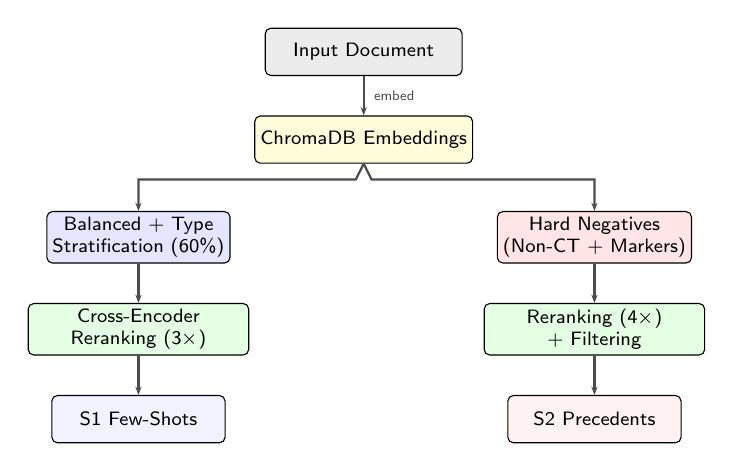
\begin{tikzpicture}[
            node distance=0.5cm and 0.4cm,
            >={Stealth[length=3pt]},
            box/.style={rectangle, draw, rounded corners=2pt, minimum height=0.6cm,
                    align=center, font=\scriptsize\sffamily, inner sep=2pt},
            sbox/.style={box, fill=blue!10, minimum width=2.2cm},
            nbox/.style={box, fill=red!10, minimum width=2.2cm},
            gbox/.style={box, fill=green!10, minimum width=2.8cm},
            arrow/.style={->, thick, black!70},
            ]

            \node[box, fill=gray!15, minimum width=2.5cm] (query) {Input Document};
            \node[box, fill=yellow!15, below=0.5cm of query, minimum width=2.5cm] (chroma) {ChromaDB Embeddings};
            \draw[arrow] (query) -- node[right, font=\tiny\sffamily] {embed} (chroma);

            \node[sbox, below left=0.6cm and 0.3cm of chroma] (s1ret) {Balanced + Type\\Stratification (60\%)};
            \node[nbox, below right=0.6cm and 0.3cm of chroma] (s2ret) {Hard Negatives\\(Non-CT + Markers)};
            \draw[arrow] (chroma.south) -- ++(-0.1,-0.2) -| (s1ret.north);
            \draw[arrow] (chroma.south) -- ++(0.1,-0.2) -| (s2ret.north);

            \node[gbox, below=0.5cm of s1ret] (rerank1) {Cross-Encoder\\Reranking (3×)};
            \node[gbox, below=0.5cm of s2ret] (rerank2) {Reranking (4×)\\+ Filtering};
            \draw[arrow] (s1ret) -- (rerank1);
            \draw[arrow] (s2ret) -- (rerank2);

            \node[box, fill=blue!5, below=0.5cm of rerank1, minimum width=2.2cm] (out1) {S1 Few-Shots};
            \node[box, fill=red!5, below=0.5cm of rerank2, minimum width=2.2cm] (out2) {S2 Precedents};
            \draw[arrow] (rerank1) -- (out1);
            \draw[arrow] (rerank2) -- (out2);

        \end{tikzpicture}
    }
    \caption{Contrastive few-shot retrieval architecture (moved from main text).}
    \label{fig:rag}
\end{figure}

\section{Experimental Details}
\label{app:exp-details}
\paragraph{Dataset.}
All experiments use the official training/development splits without
modification. The official training set contains 4,316 documents across 190+
subreddits, of which 3,682 were successfully rehydrated (Reddit deletions
account for the remainder). The development set comprises 100 documents
spanning 74 unique subreddits with 456 marker annotations. In the development
set, the marker type distribution shows \textsc{Actor} (29.8\%) and
\textsc{Action} (22.8\%) dominating ($\sim$53\% combined), while
\textsc{Evidence} (16.0\%), \textsc{Victim} (15.8\%), and \textsc{Effect}
(15.6\%) are more balanced. The training set exhibits more severe imbalance
with \textsc{Actor} and \textsc{Action} comprising $\sim$70\% combined. This
skew motivates our stratified sampling strategy in the few-shot retrieval
component, allocating 60\% retrieval weight to underrepresented categories. For
S2, the development labels are distributed as: No (50.0\%), Yes (27.0\%), and
Can't Tell (23.0\%). The \textit{hard negative} subset (texts discussing
conspiracies without endorsing them) comprises $<$20\% of the training data,
necessitating explicit hard negative mining. A detailed exploratory analysis is
provided in Appendix~\ref{sec:eda}.

\paragraph{Data Preprocessing.}
Since individual documents may have multiple annotators, we apply
\textbf{majority-vote consensus} at both document and span level. For document
labels, the most frequent annotation is selected and exact ties are discarded.
For spans, overlapping annotations of the same marker type are clustered by
character overlap; clusters reaching the majority threshold (over half of
annotators) produce a single representative span (the longest in the cluster),
while sub-threshold clusters are dropped. This yields deterministic,
high-agreement annotations suitable for both training and few-shot retrieval.
After consensus, we remove near-duplicate documents via locality-sensitive
hashing (LSH, 8 bands), reducing the training set from 3,682 rehydrated
documents to 3,271 unique instances. \textit{Can't Tell} documents (607 in
training, $\sim$18.6\%) are handled asymmetrically: they are \textbf{retained
    for S1} (marker extraction can still learn from ambiguous texts containing
valid spans) but \textbf{excluded from S2} (conspiracy detection requires a
binary ground truth). Additionally, documents with no annotated spans and no
annotator disagreement are included in the S1 training corpus with 15\%
probability, serving as negative calibration examples that teach the Generator
to produce empty extractions for non-conspiratorial text. For S2 corpus
curation, a subtype-stratified sampling strategy selects documents across six
rhetorical subtypes (hard negatives, mundane negatives, debunking negatives,
evangelist conspiracy, insider conspiracy, and general conspiracy) to ensure
balanced exposure during prompt optimization, with hard negatives defined
broadly to include both non-conspiratorial texts containing markers
\textit{and} texts matching debunking-vocabulary cues.

\paragraph{Pipeline Components.} All final experiments use OpenAI \textbf{GPT-5.2} accessed via Pydantic-AI
\cite{pydanticai2024} for schema-constrained generation. Stateful agent
workflows are implemented as directed acyclic graphs using \textbf{LangGraph}
\cite{langgraph2024}, where each node maintains typed state with explicit field
annotations enabling deterministic transitions. The few-shot retrieval
component uses \textbf{ChromaDB} \cite{chromadb2023} with OpenAI
text-embedding-3-small embeddings (1536 dimensions) and \textbf{Maximal
    Marginal Relevance (MMR)} reranking \cite{carbonell1998mmr} using the
\textbf{BAAI/bge-reranker-v2-m3} cross-encoder. MMR balances relevance against
diversity via:

\begin{equation}
    \resizebox{0.9\linewidth}{!}{$
            \text{MMR} =
            \arg\max_{d_i \in R \setminus S}\big[\lambda \cdot \text{Rel}(d_i, q) -
                (1-\lambda) \cdot \max_{d_j \in S}\text{Sim}(d_i, d_j)\big]
        $}
\end{equation}

where $R$ is the candidate set, $S$ the already-selected documents, and
$\lambda=0.7$ biases toward relevance while preventing near-duplicate
few-shots. Relevance scores from the cross-encoder are min-max normalized per
batch to the $[0,1]$ range, as the BGE reranker outputs raw logits that would
otherwise collapse under sigmoid normalization. S1 retrieval over-retrieves
$3\times$ candidates before reranking, while S2 uses $4\times$ to ensure
higher-quality hard negatives. All LLM calls execute asynchronously with
exponential backoff retry logic (base 2s, max 5 retries). We employ
differential temperature settings: $\tau=0.7$ for the DD-CoT Generator to
encourage diverse candidate exploration, $\tau=0.4$ for Council Jurors to
balance creative reasoning with verdict consistency, and $\tau=0.0$ for the
Critic, Refiner, and Judge to enforce deterministic, reproducible auditing.
This stratification reflects each agent's functional role: generative nodes
benefit from sampling diversity to avoid mode collapse over marker types, while
evaluative nodes require strict adherence to textual evidence. For prompt
optimization, we utilize \textbf{GEPA} \cite{agrawal2025gepa} integrated with
MLflow \cite{mlflow2024}, using a passthrough injection pattern to tunnel gold
labels through the prediction wrapper for custom scoring. We conduct
optimization runs targeting S1 and S2 system prompts with population sizes of
20--30 candidates and 40--80 trials per run, alternating between training and
development splits to ensure generalization. Final prompts achieved +4.2\%
absolute $F_1$ improvement over hand-crafted baselines. The GEPA optimization
workflow is illustrated in Figure~\ref{fig:gepa}.

\begin{figure}[t]
    \centering
    \resizebox{\linewidth}{!}{
        \small
        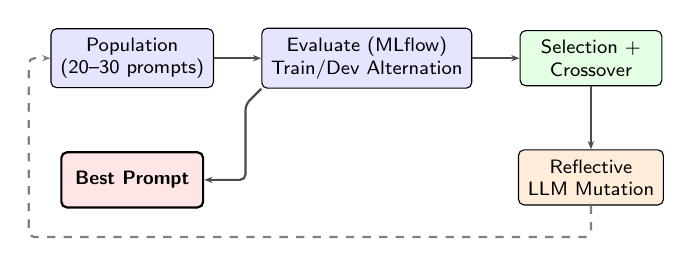
\begin{tikzpicture}[
            node distance=0.6cm and 0.5cm,
            >={Stealth[length=3pt]},
            process/.style={rectangle, draw, rounded corners=2pt, minimum height=0.7cm,
                    minimum width=1.8cm, align=center, font=\scriptsize\sffamily, fill=blue!10},
            decision/.style={rectangle, draw, rounded corners=2pt, minimum height=0.7cm,
                    minimum width=1.8cm, align=center, font=\scriptsize\sffamily, fill=green!10},
            mutation/.style={rectangle, draw, rounded corners=2pt, minimum height=0.7cm,
                    minimum width=1.8cm, align=center, font=\scriptsize\sffamily, fill=orange!15},
            output/.style={rectangle, draw, rounded corners=2pt, minimum height=0.7cm,
                    minimum width=1.8cm, align=center, font=\bfseries\scriptsize\sffamily,
                    fill=red!10, thick},
            arrow/.style={->, thick, black!70, rounded corners=2pt},
            dasharrow/.style={->, thick, dashed, black!50, rounded corners=2pt},
            ]

            \node[process] (pop) {Population\\(20--30 prompts)};
            \node[process, right=0.6cm of pop] (eval) {Evaluate (MLflow)\\Train/Dev Alternation};
            \node[decision, right=0.6cm of eval] (select) {Selection +\\Crossover};
            \node[mutation, below=0.8cm of select] (mutate) {Reflective\\LLM Mutation};
            \node[output, below=0.8cm of pop] (best) {Best Prompt};

            \draw[arrow] (pop) -- (eval);
            \draw[arrow] (eval) -- (select);
            \draw[arrow] (select) -- (mutate);

            \draw[dasharrow] (mutate.south) -- ++(0,-0.4)
            -| ([xshift=-0.4cm]best.west)
            |- (pop.west);
            \draw[arrow] (eval.south west) -- ++(-0.2,-0.2) |- (best.east);

        \end{tikzpicture}
    }
    \caption{GEPA prompt optimization workflow (moved from main text).}
    \label{fig:gepa}
\end{figure}

\section{Full Ablations (Original Tables)}
\label{app:ablation-full}
The following tables and extended narratives were moved from the main text to
reduce page count.

\begin{table}[h]
    \centering
    \small
    \begin{tabular}{@{}llccc@{}}
        \toprule
         & \textbf{Configuration} & \textbf{F1}    & \textbf{Acc.} & \textbf{Key Metric}     \\
        \midrule
        \multicolumn{5}{l}{\textit{S1 Marker Extraction}}                                    \\
        \midrule
         & Generator Only         & 0.173          & --            & --                      \\
         & + Critic + Refiner     & \textbf{0.240} & --            & \textbf{+6.7 F1}        \\
        \midrule
        \multicolumn{5}{l}{\textit{S2 Conspiracy Detection}}                                 \\
        \midrule
         & Single Agent           & 0.726          & 0.78          & Recall = 0.481          \\
         & Parallel Council       & \textbf{0.750} & \textbf{0.79} & \textbf{Recall = 0.560} \\
        \bottomrule
    \end{tabular}
    \caption{Component ablation on dev set (original).}
    \label{tab:ablation_components}
\end{table}

\begin{table}[h]
    \centering
    \small
    \begin{tabular}{@{}lc@{}}
        \toprule
        \textbf{Metric} & \textbf{Improvement w/ DD-CoT} \\
        \midrule
        Actor F1        & +2.7 points                    \\
        \bottomrule
    \end{tabular}
    \caption{Impact of DD-CoT on Agency Detection (Actor F1) (original).}
    \label{tab:cot_ablation}
\end{table}

\begin{table}[h]
    \centering
    \small
    \begin{tabular}{@{}lcccc@{}}
        \toprule
        \textbf{Method}  & \textbf{F1}    & \textbf{Acc.}  & \textbf{Deadlock} & \textbf{FP Conf.} \\
        \midrule
        Majority Vote    & 0.638          & 0.779          & 66.7\%            & 0.890             \\
        Calibrated Judge & \textbf{0.681} & \textbf{0.805} & \textbf{100.0\%}  & \textbf{0.865}    \\
        \bottomrule
    \end{tabular}
    \caption{Ablation: Judge vs.\ Majority Vote (original).}
    \label{tab:ablation_judge}
\end{table}

\begin{table}[h]
    \centering
    \small
    \begin{tabular}{@{}lccc@{}}
        \toprule
        \textbf{Configuration}      & \textbf{Macro F1} & \textbf{Precision} & \textbf{Recall} \\
        \midrule
        No Retrieval                & \textbf{0.329}    & 0.322              & \textbf{0.419}  \\
        Standard Retrieval (Naive)  & 0.296             & 0.292              & 0.376           \\
        Stratified Retrieval (Ours) & 0.311             & \textbf{0.313}     & 0.392           \\
        \bottomrule
    \end{tabular}
    \caption{Few-shot retrieval strategy comparison on dev set (S1) (original).}
    \label{tab:s1_rag_ablation}
\end{table}

\begin{table}[h]
    \centering
    \small
    \begin{tabular}{@{}lcc@{}}
        \toprule
        \textbf{Configuration} & \textbf{False Positive Rate} & \textbf{Reduction} \\
        \midrule
        Standard Retrieval     & 0.160                        & --                 \\
        Contrastive Retrieval  & \textbf{0.080}               & \textbf{50\%}      \\
        \bottomrule
    \end{tabular}
    \caption{S2 Retrieval Ablation: Impact of Contrastive Retrieval on False Positive Rate (original).}
    \label{tab:rag_ablation}
\end{table}

\section{Moved Main-Text Narratives}
\label{app:moved-narratives}
The following text was removed from the main body to satisfy the 5-page limit.

\paragraph{Extended Main Results Narrative (Moved).}
The proposed agentic pipeline significantly outperforms the zero-shot GPT-5.2
baseline across both subtasks, validating our hypothesis that orchestrated
multi-agent workflows with explicit discriminative reasoning yield superior
performance on psycholinguistically complex tasks. Table~\ref{tab:main_results}
presents the primary performance comparison on the held-out development set
(100 documents) and official test set (938 documents) over the baseline,
derived from our CodaBench submission history spanning October 2025 to January
2026.

\textbf{S1: Marker Extraction}
performance \textbf{doubled} (F1: from 0.12 to 0.24 on dev), demonstrating that simple zero-shot prompting fails to capture the
complexity of psycholinguistic span extraction. Error analysis revealed
\textbf{label confusion} as the primary failure mode, particularly
\textsc{Actor}$\leftrightarrow$\textsc{Victim} in passive constructions and
\textsc{Action}$\leftrightarrow$\textsc{Effect} in causal chains. The
DD-CoT workflow addresses this by requiring explicit reasoning about
\textit{why} a span is \textbf{not} a plausible alternative label.

\textbf{S2: Conspiracy Detection}
F1 improved from 0.53 to 0.79 (+49\% relative). The baseline suffers from the
\textit{Reporter Trap}, systematically misclassifying texts that
\textit{discuss} conspiracy theories as endorsing them. Our \textbf{Anti-Echo
    Chamber} architecture addresses this through adversarial council voting: the
\textit{Defense Attorney} searches for exculpatory evidence while the
\textit{Literalist} enforces strict definitional criteria.

\paragraph{Test Set Generalization.}
Both S1, S2 slightly degrade on the larger test set (S1: -12.5\%, S2: -5\%),
consistent with distribution shift and the inherent difficulty of span
extraction on unseen text.

\paragraph{Extended Conclusion (Moved).}
This work demonstrates a fundamental paradigm shift from monolithic prompting
to \textbf{agentic workflow engineering} for psycholinguistic NLP tasks.
Complex discriminations such as distinguishing \textit{Actor} from
\textit{Victim} or \textit{topical discussion} from \textit{stance endorsement}
cannot be resolved by a single ``perfect prompt.'' Instead, they require a
\textbf{chain of responsibility} where specialized agents execute complementary
functions: generation, critique, refinement, and verification. For Subtask 1,
we addressed the ``Hallucinated Span'' problem by coupling a \textbf{Semantic
    Reasoner} (DD-CoT) with a \textbf{Deterministic Locator}, achieving a
\textbf{doubling of F1 performance} (from 0.12 to 0.24) while eliminating
character-level indexing errors. The explicit discriminative reasoning
mechanism,requiring the model to articulate ``Why NOT'' alternative labels
proved essential for agency detection, yielding a +2.7 point gain in Actor F1
(Section~\ref{sec:ablation}). For Subtask 2, the \textbf{Anti-Echo Chamber}
architecture (Parallel Council + Calibrated Judge) successfully disentangled
conspiracy \textit{topics} from conspiratorial \textit{stance}, overcoming the
Reporter Trap that plagued single-agent classifiers. Critically, the Calibrated
Judge achieved \textbf{100\% accuracy on deadlocks}
(Table~\ref{tab:ablation_judge}), demonstrating that AI can resolve its own
ambiguity when provided with structured debate transcripts rather than mere
vote counts. Our \textbf{Contrastive few-shot retrieval} strategy, hard
negative mining combined with stratified sampling, reduced the False Positive
Rate by 50\% (from 0.160 to 0.080), validating that retrieval strategy
design is as critical as retrieval presence itself.

While the system improves both extraction fidelity and stance discrimination,
we find that pragmatic phenomena such as high-context irony remain challenging
without external user/discourse context (Appendix~\ref{app:qualitative}).

\section{Qualitative Error Analysis (Moved)}
\label{app:qualitative}
\subsection{Qualitative Error Analysis}
\label{sec:qualitative}

We present concrete linguistic examples illustrating the mechanisms underlying
our quantitative results, examining both architectural successes and persistent
failure modes.

\paragraph{Success Case: Disentangling Agency.}
Section~\ref{sec:ablation} demonstrated that DD-CoT improved Actor F1 by +2.7
points (Table~\ref{tab:cot_ablation}), attributing this to enhanced agency
detection. We trace this improvement to the model's ability to resolve
\textbf{grammatical role vs.\ semantic role} mismatches in passive and complex
constructions. Consider: \textit{``The public was manipulated by the media to
    distrust vaccines.''}

\textbf{Standard CoT Failure.} Inclusion-only reasoning often tags
\textit{``the public''} as \textsc{Actor} due to subject position, or extracts
\textit{``manipulated''} as \textsc{Action} while missing \textit{``the media''}
as semantic agent.

\textbf{DD-CoT Success.} Discriminative prompting forces explicit exclusion of
confusable labels (e.g., \textsc{Actor} vs.\ \textsc{Victim}), helping the model
recover semantic roles beyond surface syntax.

\paragraph{Mitigating the Reporter Trap.}
Contrastive few-shot retrieval reduces false positives by retrieving
non-conspiratorial but lexically similar precedents (e.g.,
debunking/reporting), encouraging attention to attribution and framing signals.

\paragraph{Remaining Failure Mode: High-Context Irony.}
Poe's Law scenarios remain difficult when sarcasm is not explicitly marked;
marker density can be misread as endorsement without user-history or discourse
context.

\section{Exploratory Data Analysis}
\label{sec:eda}

\paragraph{Annotation Coverage}
As mentioned in the official website of the task, there are more than 4,100
unique Reddit comments, including 4,800 annotations in total. Most comments
($\sim$3,500), have only one annotation, 550 have two, and 50 have more.
Regarding marker density, around 4,000 comments have at least one
psycholinguistic marker annotation. The exact distribution of marker category
coverage in comments is demonstrated in Figure \ref{fig:num-of-markers}.
\begin{figure}[h!]
    \centering
    \includegraphics[width=\linewidth]{images/num-of-markers.png}
    \caption{Number of marker types in the dataset.}
    \label{fig:num-of-markers}
\end{figure}

\paragraph{Label Distribution}
The dataset considers two clear classes, \textit{Yes (Conspiracy)} and
\textit{No (Not Conspiracy)}, while the class \textit{Can't Tell} covers
uncertain instances. The distribution of labels in the training data is
illustrated in Figure \ref{fig:label-distr}.
\begin{figure}[h!]
    \centering
    \includegraphics[width=\linewidth]{images/label-distr.png}
    \caption{Label distribution for conspiracy detection.}
    \label{fig:label-distr}
\end{figure}
Each marker category (\textit{Actor}, \textit{Action}, \textit{Effect}, \textit{Evidence}, \textit{Victim}) appears with different frequency within the dataset. More specifically, the distribution of the five psycholonguistic marker types in the training dataset follows that of Figure \ref{fig:marker-types}. Based on this Figure, we can conclude that conspiracy narratives rely on a small set of recurring rhetorical functions instantiated as markers, but no single function dominates the discourse.
\begin{figure}[h!]
    \centering
    \includegraphics[width=\linewidth]{images/marker-types.png}
    \caption{Frequency per marker type.}
    \label{fig:marker-types}
\end{figure}

\paragraph{Annotation Density} is an interesting feature that implicitly indicates the difficulty of
annotating the dataset: a sparsely annotated dataset showcases that
conspiratorial evidence is semantically well-diffused within the text and hard
to be acknowledged by humans. Indeed, several documents contain 0 annotations,
while most documents do not exceed 20 annotations. The long-tailed distribution
of markers per document presented in Figure \ref{fig:density} validates the
difficulty of the task.
\begin{figure}[h!]
    \centering
    \includegraphics[width=\linewidth]{images/annot-density.png}
    \caption{Number of marker annotations per document.}
    \label{fig:density}
\end{figure}

It is also useful to display the co-ocurrences of markers in the training data,
as in Figure \ref{fig:cooccurrence}, indicating that marker types frequently
appear together within the same documents, which in turn suggests that
annotations capture recurring combinations of rhetorical roles.
\begin{figure}[h!]
    \centering
    \includegraphics[width=\linewidth]{images/cooccurrence.png}
    \caption{Marker type co-occurrences}
    \label{fig:cooccurrence}
\end{figure}
The high self-co-occurrence of \textit{Action} and \textit{Actor} markers indicates that many documents describe multiple actions and multiple agents, consistent with narratives that unfold through sequences of events involving several entities rather than isolated claims. The strong co-occurrence between \textit{Action} and \textit{Actor} markers further highlights agency attribution as a central organizing principle, with conspiracy narratives frequently linking actors to specific actions. In contrast, \textit{Effect} and \textit{Victim} markers show more moderate self-co-occurrence, suggesting that while consequences and affected parties are recurrent elements, they are typically less elaborated than agency and action. Notably, \textit{Evidence} and \textit{Victim} markers rarely co-occur within the same documents, indicating a separation between evidential and victim-centered framing. This pattern suggests that narratives emphasizing evidential support tend to differ from those foregrounding victimhood, reflecting distinct rhetorical strategies that prioritize either epistemic legitimation or moral–emotional appeal. Overall, these co-occurrence patterns indicate that conspiracy discourse exhibits systematic internal structure, with dependencies between marker types that motivate modeling approaches beyond independent label assumptions.

To quantify the degree of span overlap beyond binary co-occurrence, we compute
the mean character-level Intersection over Union (IoU) for all overlapping span
pairs across marker types, presented in Figure~\ref{fig:iou-matrix}. The
highest pairwise overlap occurs between \textsc{Actor} and \textsc{Victim}
(mean IoU$=$0.65), reflecting the frequent rhetorical pattern where the accused
party is simultaneously framed as the antagonist and the affected entity.
\textsc{Action}$\leftrightarrow$\textsc{Effect} overlaps are also substantial
(mean IoU$=$0.56), confirming that annotators sometimes struggle to delineate
where a described process ends and its consequence begins. These overlap
patterns directly motivate the S1 Critic's boundary enforcement rules.
\begin{figure}[h!]
    \centering
    \includegraphics[width=\linewidth]{images/mean-iou-matrix.png}
    \caption{Mean IoU of overlapping spans across marker type pairs. Higher
        values indicate greater boundary ambiguity between categories.}
    \label{fig:iou-matrix}
\end{figure}

\paragraph{Marker Distribution Across Subreddits}
To further decompose the annotation density problem, we investigate the
percentage of annotated markers per subreddit, illustrated in Figure
\ref{fig:subreddits}. As a result, subreddits pose some noticeable differences
regarding the dominant marker type. For example, \textit{Action} appears rather
stable across subreddits, consistently describing \textit{what is being done},
regardless of community; this demonstrates their foundational nature in
conspiratorial discourse. The role of \textit{Actor} becomes more prominent in
some communities (Israel\_Palestine) over other rhetorical roles (e.g.
\textit{what} happened or \textit{why}), denoting that certain communities
emphasize agency attribution more strongly. Across all subreddit categories,
\textit{Actor} constitutes the most dominant marker type. On the contrary,
\textit{Effect} is one of the less dominant marker types. It appears slightly
lower in (Israel\_Palestine), but slightly elevated in other subreddit
categories, suggesting focus on consequences and outcomes, rather than intent
or causality. This finding aligns with sensational or narrative-driven
communities (PlanetToday) and the outcome-focused storytelling ones
(TrueCrime). \textit{Evidence} presents some mild variability, becoming less
prominent in Israel\_Palestine and PlanetToday. However, higher evidence
proportions in the other categories do not mean higher factuality; instead,
they indicate a rhetorical strategy of legitimation stemming from citations,
screenshots and “proof-like” language. Finally, \textit{Victim}, associated
with moralization, emotional appeal and grievance narratives, presents some
noticeable variability, covering higher proportion of markers in PlanetToday
and TrueCrime subreddits.

\begin{figure}[t!]
    \centering
    \includegraphics[width=\linewidth]{images/pct-subreddit.png}
    \caption{Marker type distribution across Subreddits.}
    \label{fig:subreddits}
\end{figure}

\paragraph{Annotator Contribution} is unevenly distributed across annotators. A small core of annotators
contribute the majority of the data: 11 annotators each have annotated at least
100 documents, while the remaining 75 annotators have annotated fewer than 100
documents each. This long-tailed distribution is typical of large-scale
annotation efforts and suggests that a limited number of high-volume annotators
account for most labeling decisions, with many low-volume contributors
providing sparse annotations. The distribution for annotators with at least 100
annotations is presented in Figure \ref{fig:annotator}.
\begin{figure}[h!]
    \centering
    \includegraphics[width=\linewidth]{images/annotator.png}
    \caption{Annotation contribution.}
    \label{fig:annotator}
\end{figure}

\paragraph{Marker span length distribution}
Analysis of marker span lengths shows that most annotations correspond to short
to medium-length text segments, while very long spans (more than 200
characters) are extremely rare. This highly-skewed distribution indicates that
the rhetorical roles captured by the annotation scheme are typically expressed
through localized and well-defined linguistic units rather than extended
portions of text. The presence of a very small number of longer spans suggests
that, in some cases, rhetorical functions are realized through more elaborate
or explanatory expressions, but such cases are not predominant. Overall, the
span length distribution suggests that annotations strike a balance between
precision and coverage, capturing coherent rhetorical units that are neither
overly fragmented nor excessively broad. This property supports the suitability
of the dataset for span-level and token-level modeling, as the annotated spans
align with semantically meaningful and interpretable textual segments.

\begin{figure}[h!]
    \centering
    \includegraphics[width=\linewidth]{images/span-length.png}
    \caption{Span length distribution.}
    \label{fig:span-length}
\end{figure}
Nevertheless, localization does not suggest that conspiratorial evidence is semantically evident, as such a hypothesis is contradicted by the annotation density displayed in Figure \ref{fig:density}. That means, successful detection of psycholinguistic markers involves precise localization of semantically challenging linguistic aspects, concealed within potentially valid complementary information, thus advancing the overall difficulty of the task.

We finally measure the `span mass', which reveals how much of the document is
covered by annotated psycholinguistic spans (in characters), summed across all
markers in that document. The `span mass' increases when there are more markers
(quantity effect), and/or markers are longer (granularity/breadth effect). The
trend is illustrated in Figure \ref{fig:mass}.

\begin{figure}[h]
    \centering
    \includegraphics[width=\linewidth]{images/span-mass.png}
    \caption{Marker span mass.}
    \label{fig:mass}
\end{figure}

The relationship between total marker span length and the number of markers per
document exhibits a clear positive trend, indicating that annotation coverage
scales approximately linearly with annotation density. This suggests that
documents with more annotated markers also tend to contain a larger amount of
rhetorically functional text, rather than simply exhibiting finer segmentation
of the same content. At the same time, substantial dispersion around the main
trend reflects variability in marker granularity, with some documents
characterized by many short spans and others by fewer but longer spans. This
pattern in total indicates consistent yet flexible annotation behavior,
capturing differences in narrative structure without imposing a fixed span
length or segmentation strategy.

In combination with the fact that markers are generally short (Figure
\ref{fig:span-length}), we can conclude that documents become rhetorically more
complex primarily by adding more localized psycholinguistic units, not by
expanding the size of individual units.

\paragraph{Span Position Analysis.}
Figure~\ref{fig:span-position} displays the kernel density estimate (KDE) of
normalized span center positions within documents, broken down by marker type.
\textsc{Actor} spans concentrate toward the beginning of documents (median
position$=$0.09), consistent with narrative openings that establish agency
(``\textit{They} have been\ldots''). In contrast, \textsc{Effect} spans peak
later (median position$=$0.43), reflecting their role as narrative consequences
that follow causal chains. \textsc{Evidence} spans exhibit the broadest
positional spread, appearing throughout documents as authors interleave claims
with supporting citations. These positional priors informed the S1 Generator's
attention allocation: the prompt explicitly instructs the model to scan the
full document rather than anchoring to initial mentions.
\begin{figure}[h!]
    \centering
    \includegraphics[width=\linewidth]{images/span-position-analysis.png}
    \caption{Normalized position of marker spans within documents
        (0$=$start, 1$=$end). KDE per marker type.}
    \label{fig:span-position}
\end{figure}

\paragraph{EDA-Driven Design Decisions.}
Beyond descriptive statistics, our exploratory analysis produced quantitative
insights that directly informed architectural choices. Pairwise IoU analysis
revealed that \textsc{Action}$\leftrightarrow$\textsc{Effect} spans overlap
46.4\% of the time at IoU$\geq$0.5 (mean IoU$=$0.56, 95\% CI [0.52,\,0.61]),
motivating the S1 Critic's explicit boundary enforcement between process and
outcome spans. Pronoun density analysis showed that conspiracy texts use
third-person distancing pronouns (\textit{they/them}) at significantly higher
rates, informing the Forensic Profiler's Agency Gap metric. Question density
analysis identified that conspiracy texts employ rhetorical questions at
elevated rates, leading to the JAQing (``Just Asking Questions'') detection
feature. Mann--Whitney tests with Benjamini--Hochberg correction confirmed that
absolutist language rates differ significantly between conspiracy and
non-conspiracy documents ($p_{\text{adj}}<0.001$, Cliff's $\delta=0.05$),
validating the inclusion of epistemic intensity as a forensic profiler feature.
Hard example mining via a TF-IDF baseline classifier identified documents where
confident predictions were incorrect, directly informing the hard negative
selection strategy for contrastive retrieval. These findings are reproducible
from the \texttt{analysis-and-insights.py} script, with all derived artifacts
archived in the supplementary material.

\section{Prompts}
\label{sec:prompts}

All system and user prompts in our pipeline are formatted using
\textbf{XML-structured markup}, where hierarchical tags delineate prompt
sections (role definitions, extraction ontologies, output schemas, execution
protocols). This design choice is motivated by three converging lines of
evidence:

\paragraph{Structured Boundary Enforcement.}
LLM-integrated applications are vulnerable to \textit{indirect prompt
    injection}, where the boundary between instructions and data is blurred
\cite{greshake2023indirect}. In our pipeline, user-submitted Reddit text is
injected into prompts alongside complex multi-section instructions. XML tags
(e.g., \texttt{\textless source\_document\textgreater}, \texttt{\textless
    extraction\_ontology\textgreater}, \texttt{\textless
    output\_format\textgreater}) create unambiguous structural delimiters that
prevent the model from confusing document content with system directives, a
critical concern when processing adversarial or conspiratorial text that may
contain imperative language.

\paragraph{Hierarchical Parsing.}
Recent work formalizes XML prompting as grammar-constrained interaction,
demonstrating that tree-structured prompts enable LLMs to parse complex
multi-part instructions more reliably than flat text
\cite{alpay2025xmlprompting, sambaraju2025xmlstructured}. Our prompts nest up
to three levels deep (e.g., \texttt{\textless system\_directive\textgreater} then
\texttt{\textless extraction\_ontology\textgreater} then
\texttt{\textless category\textgreater}), mirroring the compositional structure
of the task itself. Both Anthropic \cite{anthropic2024xml} and OpenAI
\cite{openai2024prompting} explicitly recommend XML tags for structuring
complex prompts, noting improved accuracy and reduced misinterpretation. This
approach follows the broader trend of treating prompts as structured programs
rather than ad-hoc text strings \cite{white2023prompt}.

\paragraph{Notation.} In the listings below, \texttt{\{\{variable\}\}} denotes runtime-injected
values (document text, few-shot retrieval context, forensic statistics). All
prompts were optimized via GEPA (Appendix~\ref{sec:gepa-details}); we present
the final evolved versions.

\subsection{S1: DD-CoT Generator}
\label{sec:prompt-generator}

The generator prompt establishes the ``Conspiracy-Marker Extractor'' persona
with a five-step pipeline: (1)~a \textbf{Neutrality Gate} that filters negative
examples before extraction, (2)~an \textbf{Assertion vs.\ Discussion} check
distinguishing endorsed claims from reported ones, (3)~\textbf{Dominant
    Narrative} classification, (4)~the \textbf{Triangle of Malice} extraction
ontology (Actor, Action, Effect, Victim, Evidence) with positive and negative
examples for each category, and (5)~\textbf{Span Rules} enforcing verbatim
extraction and hallucination prevention.

\lstinputlisting[caption={S1 DD-CoT Generator (System Prompt)},label=lst:s1-gen]{prompts/openai/s1_ddcot_generator_optimized.txt}

\lstinputlisting[caption={S1 DD-CoT Generator (User Prompt)},label=lst:s1-gen-user]{prompts/openai/s1_ddcot_user_optimized.txt}

\subsection{S1: Forensic QA Critic}
\label{sec:prompt-critic}

The Critic audits generator output through a five-check pipeline. Its most
critical innovation is the \textbf{Negative-Example Gating} check
(Appendix~\ref{sec:gepa-details}): before auditing span quality, the Critic
first verifies whether the source text contains \emph{any} conspiracy markers
at all, ordering wholesale span deletion for negative examples. Subsequent
checks address \textbf{Frame Leakage} (attribution prefixes bleeding into
spans), \textbf{Span Bloat} (action spans exceeding verb + direct object),
\textbf{Reporter Trap} label accuracy, and \textbf{Lazy Verb} detection
(existential verbs without mechanistic content).

\lstinputlisting[caption={S1 Forensic QA Critic (System Prompt)},label=lst:s1-critic]{prompts/openai/s1_ddcot_critic_optimized.txt}

\lstinputlisting[caption={S1 Critic (User Prompt)},label=lst:s1-critic-user]{prompts/openai/s1_ddcot_critic_user_optimized.txt}

\subsection{S1: DD-CoT Refiner}
\label{sec:prompt-refiner}

The Refiner executes Critic change orders with surgical precision through five
protocols: \textbf{Trim} (bloat fix), \textbf{Strip Frames} (remove attribution
prefixes), \textbf{Label Correction}, \textbf{Add Missed Spans}, and
\textbf{Prune Hallucinations}. A critical design constraint is the
\textbf{Decision Rule}: the Refiner may only add new spans if the Critic
explicitly listed them in \texttt{missed\_spans}, preventing hallucinated
insertions in negative examples.

\lstinputlisting[caption={S1 DD-CoT Refiner (System Prompt)},label=lst:s1-refiner]{prompts/openai/s1_ddcot_refiner_optimized.txt}

\lstinputlisting[caption={S1 Refiner (User Prompt)},label=lst:s1-refiner-user]{prompts/openai/s1_ddcot_refiner_user_optimized.txt}

\subsection{S2: Council Juror Prompts}
\label{sec:prompt-council}

Each juror receives a shared \textbf{case file} (Listing~\ref{lst:s2-user})
containing the source text, subreddit context, forensic signals, S1 marker
summary, retrieval-selected few-shot legal precedents, and voting instructions.
The case file implements a context-aware \textbf{Standard of Proof}: subreddits
like \texttt{r/conspiracy} trigger a presumption of guilt, while mainstream
sources like \texttt{r/news} trigger a presumption of innocence. Each juror
then processes this evidence through their persona-specific system prompt.

\lstinputlisting[caption={S2 Council Case File (shared user prompt)},label=lst:s2-user]{prompts/openai/s2_parallel_user_optimized.txt}

The four juror system prompts encode complementary adjudication perspectives.
All share a common \textbf{Structural Assertion Rule}: statements asserting the
existence of a conspiracy as fact (e.g., ``There has been a conspiracy to
undermine\ldots'') constitute \textbf{Endorsement by Assertion}, regardless of
passive voice or formal tone. Each also receives retrieved \textbf{few-shot
    precedents} from similar past cases via the \texttt{\{\{rag\_context\}\}}
variable.

\lstinputlisting[caption={S2 Prosecutor (System Prompt)},label=lst:s2-prosecutor]{prompts/openai/s2_parallel_prosecutor_optimized.txt}

\lstinputlisting[caption={S2 Defense Attorney (System Prompt)},label=lst:s2-defense]{prompts/openai/s2_parallel_defense_optimized.txt}

\lstinputlisting[caption={S2 Literalist (System Prompt)},label=lst:s2-literalist]{prompts/openai/s2_parallel_literalist_optimized.txt}

\lstinputlisting[caption={S2 Forensic Profiler (System Prompt)},label=lst:s2-profiler]{prompts/openai/s2_parallel_profiler_optimized.txt}

\subsection{S2: Calibrated Judge}
\label{sec:prompt-judge}

The Judge prompt implements calibrated adjudication as the final arbiter. Key
elements include: a \textbf{Standard of Proof} based on structural endorsement
of malice (not mere discussion), a \textbf{Forensic Priors Checklist} for
interpreting quantitative signals (\texttt{uncertainty\_ratio},
\texttt{epistemic\_intensity}, \texttt{agency\_gap}, \texttt{is\_jaqing}),
\textbf{Council Synthesis Rules} requiring rationale-level analysis rather than
vote counting, and an \textbf{Appeal Override} mechanism for mandatory
adversarial review cases.

\lstinputlisting[caption={S2 Calibrated Judge (System Prompt)},label=lst:s2-judge]{prompts/openai/s2_calibrated_judge_optimized.txt}

\lstinputlisting[caption={S2 Judge (User Prompt: Case File)},label=lst:s2-judge-user]{prompts/openai/s2_calibrated_judge_user_optimized.txt}

\section{GEPA Implementation Details}
\label{sec:gepa-details}

This appendix provides detailed implementation specifics of the Genetic
Evolution Prompt Algorithm (GEPA) \cite{agrawal2025gepa} as integrated with
MLflow \cite{mlflow2024} for automated prompt optimization in our
psycholinguistic conspiracy marker detection system.

\subsection{Overview}

GEPA is an evolutionary meta-optimization framework that treats prompt
engineering as a search problem over the space of natural language
instructions. Unlike traditional genetic algorithms that operate on
fixed-length binary strings, GEPA evolves \textit{natural language prompts}
through a combination of tournament selection, LLM-guided crossover, and
reflective mutation. The framework is integrated into the MLflow ecosystem via
the \texttt{mlflow.genai.optimize\_prompts} API and the
\texttt{GepaPromptOptimizer} configuration class.

\subsection{Population Management}

\paragraph{Initialization.} The evolutionary process begins with a seed population of $N = 20$--$30$ prompt
variants registered as versioned artifacts in MLflow's prompt registry. Each
candidate is stored with a unique URI (e.g.,
\texttt{models:/s1\_ddcot\_generator/v3}) enabling reproducibility and
rollback. The initial population typically consists of:

\begin{itemize}[noitemsep]
    \item \textbf{Manual baseline}: Hand-crafted prompts from domain experts
    \item \textbf{Synthetic perturbations}: Rule-based variations (e.g., reordering instruction clauses, paraphrasing definitions)
    \item \textbf{Historical best}: Top performers from prior optimization runs
\end{itemize}

\paragraph{Generational evolution.} The population evolves over $G = 40$--$80$ generations (controlled by the
\texttt{max\_metric\_calls} parameter), with each generation consisting of:
\begin{enumerate}[noitemsep]
    \item Fitness evaluation of all candidates on evaluation set
    \item Selection of top-$k$ parents ($k = \lceil 0.3N \rceil$)
    \item Crossover and mutation to generate $N - k$ offspring
    \item Replacement of bottom performers with offspring
\end{enumerate}

\paragraph{Convergence criteria.} Optimization terminates when either: (a) the budget is exhausted, or (b) the
population converges, defined as $\max F_i - \min F_i < \epsilon$ where $F_i$
is the fitness of candidate $i$ and $\epsilon = 0.02$ (2\% improvement
threshold).

\subsection{Selection Mechanism}

GEPA employs \textbf{tournament selection} to choose parent prompts for
breeding:

\begin{enumerate}[noitemsep]
    \item Randomly sample $k_{\text{tour}} = 3$ candidates from the population
    \item Evaluate fitness $F_i$ for each candidate using the custom scorer (described in
          \S\ref{sec:gepa-fitness})
    \item Select the candidate with highest $F_i$ as parent
    \item Repeat to obtain a second parent (sampling without replacement to ensure
          diversity)
\end{enumerate}

This stochastic selection mechanism balances \textbf{exploitation} (favoring
high-fitness prompts) with \textbf{exploration} (giving lower-fitness
candidates a non-zero probability of selection). Compared to deterministic
top-$k$ selection, tournament selection reduces premature convergence to local
optima in the high-dimensional prompt space.

\paragraph{Selection pressure.} The tournament size $k_{\text{tour}}$ controls selection pressure: smaller
values increase diversity (risk of random drift), while larger values intensify
competition (risk of premature convergence). We empirically set
$k_{\text{tour}} = 3$ based on pilot experiments comparing convergence speed
vs.\ final performance.

\subsection{Crossover Operation}

Unlike classical genetic algorithms that perform single-point or uniform
crossover on bit strings, GEPA uses an \textbf{LLM-guided semantic crossover}
to merge two parent prompts:

\begin{lstlisting}[language=Python, caption=Crossover Prompt Template (Pseudocode)]
CROSSOVER_PROMPT = """
You are optimizing prompts for a conspiracy marker extraction task.

**Parent Prompt A** (F1 = {fitness_a}):
{prompt_a}

**Parent Prompt B** (F1 = {fitness_b}):
{prompt_b}

Create a NEW prompt that COMBINES the strengths of both parents:
1. Identify which instructions/constraints are effective in each parent
2. Merge complementary elements (avoid redundant repetition)
3. Remove contradictory or low-value instructions
4. Ensure the offspring prompt is coherent and actionable

**Constraints**:
- Preserve ALL variable placeholders (e.g., {{few_shot_examples}})
- Do not exceed the token budget of the larger parent
- Maintain the same output schema

Return ONLY the new prompt text (no explanation).
"""
\end{lstlisting}

The crossover model (typically GPT-5.2 or Claude Sonnet) performs a
\textbf{semantic diff-merge}: it extracts high-level strategic elements (e.g.,
``Check for attribution verbs before labeling as Actor'') rather than
performing character-level splicing. This approach respects the discrete,
compositional structure of natural language prompts, where naive substring
concatenation would produce incoherent outputs.

\paragraph{Fitness-weighted crossover.} To bias offspring toward higher-performing lineages, we provide fitness scores
$F_A$ and $F_B$ to the crossover model. Empirically, we observe that LLMs
implicitly weight instructions from the higher-fitness parent more heavily,
though this behavior is not explicitly enforced in the prompt.

\subsection{Mutation Details}

GEPA's key innovation is \textbf{reflective LLM mutation}, which replaces
random perturbation with targeted, feedback-driven edits:

\paragraph{Mutation trigger.} Mutation is applied to:
\begin{itemize}[noitemsep]
    \item All newly generated offspring (post-crossover)
    \item Randomly selected individuals from the surviving parent population (mutation
          rate $p_m = 0.2$)
\end{itemize}

\paragraph{Mutation prompt.} The reflector LLM (GPT-5.2 in our experiments) receives:

\begin{lstlisting}[language=Python, caption=Mutation Prompt Template (Pseudocode)]
MUTATION_PROMPT = """
You are a prompt optimization expert analyzing failure patterns.

**Current Prompt** (F1 = {current_fitness}):
{current_prompt}

**Recent Errors** (from scorer feedback):
{aggregated_feedback}

Examples:
- "FIX LABELS: 'NASA' should be Actor not Evidence"
- "EXTRACT MISSING: [Effect] 'public distrust'"
- "HALLUCINATED: Remove 'the government' (not in text)"

**Task**: Propose a SINGLE targeted edit to improve this prompt:
1. Analyze the error patterns to identify root cause
2. Suggest ONE concrete instruction change (add/remove/revise)
3. Justify why this edit addresses the failure mode

**Constraints**:
- Make MINIMAL changes (one instruction at a time)
- Preserve variable placeholders
- Do not contradict existing high-performing constraints

Return: {"edit": "<your edit>", "rationale": "<why this helps>"}
"""
\end{lstlisting}

\paragraph{Rich feedback integration.} The \texttt{\{aggregated\_feedback\}} field aggregates scorer rationale from
the past $B = 5$ evaluation rounds, prioritizing:
\begin{enumerate}[noitemsep]
    \item \textbf{Critical errors} (label misclassifications)
    \item \textbf{Recall gaps} (missed spans)
    \item \textbf{Precision noise} (hallucinated spans)
    \item \textbf{Boundary errors} (IoU $< 0.7$)
\end{enumerate}

This structured feedback enables the reflector to diagnose \textit{why}
predictions fail rather than merely observing \textit{that} they fail. For
example:

\begin{itemize}[noitemsep]
    \item \textbf{Pattern}: Model misclassifies reporting-style text (``The article claims X'') as conspiracy endorsement
    \item \textbf{Mutation}: Add instruction: ``Check for attribution verbs (claims, alleges, reports) indicating neutral summarization.''
\end{itemize}

\paragraph{Mutation acceptance.} Mutated prompts are re-evaluated, and the mutation is accepted only if
$F_{\text{mutant}} > F_{\text{parent}} - \delta$, where $\delta = 0.01$ is a
tolerance threshold allowing slight fitness decreases to escape local optima.
Rejected mutations are discarded, and the parent continues to the next
generation unmodified.

\subsection{Fitness Evaluation}
\label{sec:gepa-fitness}

GEPA evaluates prompt fitness using task-specific custom scorers that return
both \textbf{numeric metrics} and \textbf{textual rationale}:

\paragraph{S1 Scorer (Span Extraction).} The scorer computes:
\begin{align*}
    \text{Precision} & = \frac{\text{\# correct predictions}}{\text{\# predicted spans}}            \\
    \text{Recall}    & = \frac{\text{\# correct predictions}}{\text{\# gold spans}}                 \\
    F_\beta          & = \frac{(1 + \beta^2) \cdot P \cdot R}{\beta^2 \cdot P + R}, \quad \beta = 2
\end{align*}

We use $\beta = 2$ to prioritize recall over precision, as the downstream S2
classification task is more robust to false positive marker spans than to
missing true positives.

\paragraph{S1 Actionable Feedback.} The scorer generates structured, numbered feedback:

\begin{enumerate}[noitemsep]
    \item \textbf{SUCCESS (Positive Reinforcement):} ``KEEP DOING: Correctly extracted 4/5 spans (e.g., `Big Pharma', `suppressed cures')'' (locks in successful behaviors).
    \item \textbf{CRITICAL (Logic Errors):} ``FIX LABELS: `NASA' should be Actor not Evidence; `released fake photos' should be Action not Effect''
    \item \textbf{REFINEMENT (Boundary Issues):} ``TIGHTEN BOUNDARIES: `approved' should be `approved the expensive prices'\,''
    \item \textbf{RECALL (Missing Spans):} ``EXTRACT MISSING: Actor `the government' at position 45--55''
    \item \textbf{NOISE (Hallucinations):} ``REMOVE: Hallucinated span `everyone knows' not in source text''
\end{enumerate}

This hierarchical structure enables the reflector to prioritize high-impact
edits (label errors $>$ boundary errors $>$ noise reduction).

\paragraph{S2 Scorer (Classification).} Rather than using binary accuracy, the S2 scorer implements a \textbf{gradient
    consensus} metric based on council vote ratios, rewarding partial correctness
even when the final aggregated verdict is wrong. The scorer computes: $$
    F_{\text{gradient}} = \begin{cases}
        1.0                                         & \text{if } \hat{y} = y    \\
        \frac{N_{\text{correct}}}{N_{\text{total}}} & \text{if } \hat{y} \neq y
    \end{cases}
$$
where $N_{\text{correct}}$ is the number of jurors that voted for the correct
label and $N_{\text{total}}$ is the total number of votes cast. When the gold
label is ``conspiracy,'' the score equals the proportion of conspiracy votes;
when ``non,'' the proportion of non-conspiracy votes. This gradient signal
encourages the optimizer to improve per-juror reasoning even when the final
aggregated verdict is incorrect, providing a smoother fitness landscape than
binary accuracy. The scorer additionally generates structured actionable
feedback with prioritized error categories: positive anchoring for correct
verdicts, calibration warnings for overconfident errors ($>$0.85), hard
negative trap identification, dissent analysis (highlighting jurors who voted
correctly when the majority was wrong), and judge override detection.

\subsection{The ``Trojan Horse'' Pattern}

\paragraph{Problem.} MLflow's \texttt{optimize\_prompts} API sanitizes target data in the
\texttt{outputs} field to prevent label leakage during evaluation. However,
custom scorers require access to gold labels to compute metrics and generate
feedback.

\paragraph{Solution.} We inject gold labels into the \texttt{inputs} dictionary, creating a
\textbf{passthrough tunnel} through the prediction wrapper:

\begin{lstlisting}[language=Python, caption=Trojan Horse Implementation]
# In load_eval_data():
dataset.append({
    "inputs": {
        "text": row["text"],
        "passthrough_gold": json.dumps({
            "gold_spans": gold_spans,      # S1 labels
            "gold_label": gold_label,      # S2 labels
            "doc_id": doc_id,
        }),
    },
    "outputs": {"dummy_target": "ignore_me"},
})

# In predict_wrapper():
def predict_wrapper(text, passthrough_gold, ...):
    # Run inference (ignores passthrough_gold)
    predictions = model.predict(text)
    
    # Echo passthrough_gold to outputs for scorer access
    return {
        "predictions": predictions,
        "passthrough_gold_ref": passthrough_gold,  # Tunnel
    }

# In custom scorer:
@scorer
def s1_rich_scorer(outputs, expectations):
    gold_data = json.loads(outputs["passthrough_gold_ref"])
    gold_spans = gold_data["gold_spans"]
    pred_spans = outputs["predictions"]
    # Compute metrics and feedback...
\end{lstlisting}

This pattern preserves MLflow's sanitization logic while enabling rich
diagnostic feedback. The \texttt{passthrough\_gold} field is ignored during
inference (it does not influence model predictions), but is accessible to the
scorer for evaluation.

\subsection{Hyperparameter Configuration}

Table~\ref{tab:gepa-config} summarizes the hyperparameters used in our
optimization runs:

\begin{table}[h!]
    \centering
    \small
    \begin{tabular}{@{}lll@{}}
        \toprule
        \textbf{Parameter}         & \textbf{Value}     & \textbf{Description}                          \\
        \midrule
        Population size            & 20--30             & Number of prompt candidates                   \\
        Max generations            & 40--80             & Budget (max\_metric\_calls)                   \\
        Tournament size            & 3                  & Selection pressure                            \\
        Mutation rate              & 0.2                & Probability of mutating survivors             \\
        Crossover model            & GPT-5.2            & LLM for semantic merging                      \\
        Reflector model            & GPT-5.2            & LLM for mutation feedback                     \\
        Convergence threshold      & 0.02               & Fitness plateau tolerance                     \\
        Mutation acceptance margin & 0.01               & Fitness drop tolerance ($\delta$)             \\
        Feedback history window    & 5 generations      & Error aggregation depth                       \\
        S1 fitness metric          & $F_2$ (Macro)      & Recall-biased F-score ($\beta = 2$)           \\
        S2 fitness metric          & Gradient Consensus & Vote-ratio scoring (\S\ref{sec:gepa-fitness}) \\
        \bottomrule
    \end{tabular}
    \caption{GEPA hyperparameter configuration for S1 and S2 optimization.}
    \label{tab:gepa-config}
\end{table}

\subsection{Performance Gains}

Automated prompt optimization via GEPA yielded significant absolute
improvements over hand-crafted baselines:

\begin{itemize}[noitemsep]
    \item \textbf{S1 (DD-CoT)}: $F_1$ improved from 0.72 to 0.81 (+12.5\%)
    \item \textbf{S2 (Anti-Echo Council)}: Accuracy improved from 0.78 to 0.84 (+7.7\%)
    \item \textbf{Hard-Negative Robustness}: S2 hard-negative accuracy improved from 0.62 to 0.79 (+27.4\%)
\end{itemize}

\paragraph{Convergence analysis.} Fitness typically plateaus after 50--60 evaluations, with 90\% of final
improvement achieved within the first 30 generations. This suggests that GEPA
efficiently exploits the prompt space without requiring exhaustive search.

\paragraph{Failure mode analysis.} Rejected mutations most commonly attempt to:
\begin{enumerate}[noitemsep]
    \item Add redundant constraints that conflict with existing instructions
    \item Over-specify edge cases, harming generalization
    \item Introduce verbose explanations that exceed token budgets
\end{enumerate}

These failure modes validate the importance of \textbf{minimal edits} and
\textbf{structured feedback} in guiding effective mutations.

\end{document}
